\documentclass[fleqn,10pt,twoside]{gcb15submission}
\usepackage{url}\urlstyle{same}
\usepackage{booktabs}
\usepackage{colortbl, xcolor}

\title{signalHsmm - a novel semi-Markov model of eukaryotic signal peptides}

\author[1]{Micha\l{}  Burdukiewicz}
\author[2]{Piotr Sobczyk}
\author[1]{Pawe\l{} B\l{}a\.{z}ej}
\author[1]{Pawe\l{} Mackiewicz}
\affil[1]{University of Wroc\l{}aw, Department of Genomics, Poland}
\affil[2]{Wroc\l{}aw University of Technology, Department of Mathematics, Poland}

\keywords{Keyword1, Keyword2, Keyword3}

\begin{abstract}
The proper localization of proteins in a cell is essential to maintain their desired function. Information about the protein destination is included within the very protein in the form of short peptides called targeting signals. Ones of them are signal peptides, diverse N-terminal sequences, which are responsible for targeting of proteins to endomembrane system and their export outside the cell. Proteins equipped with signal peptides play crucial roles in metabolism, maintenance of tissue structure, immune response and regulation of other organismal functions. Moreover, the transport of proteins through the endomembrane system is important for their correct folding and posttranslational modifications. 

A common model of classical signal peptides assumes that they start with a positively charged n-region, followed by a hydrophobic h-region and a c-region ended with a cleavage site recognised by a signal peptidase. However, our studies of many protein sequences representing the wide range of diversified taxonomic organisms indicate a variability of signal peptides. Therefore, we designed a new, more univeral probabilistic model for eukaryotic signal peptides, which includes knowledge about their organisation, amino acid composition and variation.

The proposed model is based on hidden semi-Markov models (HSMMs) and use intrinsic knowledge about signal peptides. The big advantage of the algorithm is its extensibility. Using the k-mers we point how the general model can be attuned to yield not only better results, but also more information about signal peptides.

Our preliminary model has showed the largest AUC=0.98 in comparison to other software and appeared very stable in the recovery of signal peptides after training even on very small data sets. Thanks to that, our model does not need to be permanently retrained with the continuous expansion of sequence databases. It should be emphasised that our model describes signal peptides from medically significant malaria parasites Plasmodium and their relatives (AUC = 0.92) more accurately than popular programs (0.84).

\end{abstract}

\begin{document}
\flushbottom
\maketitle
\thispagestyle{empty}


\section*{Introduction}


Proteins of eukaryotes are encoded in nuclear genomes and are synthetized in ribosomes located in the cytosol or bounded by the endoplasmic reticulum. After the translation process, proteins have to be targeted to specific subcellular compartments or exported outside the cell to the extracellular environment. The proper localization of proteins is essential to perform their desired function. Information about protein destination is included within the very protein in the form of short peptides or stretches of amino acid residues called targeting or sorting signals. Ones of them are signal peptides, which are located at the N-terminus of proteins.

Signal peptides are responsible for targeting of proteins to endomembrane system, which includes endoplasmic reticulum, Golgi apparatus and endosomes. Such proteins can stay inside of these compartments, or can be inserted into cellular membranes or exported outside the cell. Proteins equipped with signal peptides constitute a substantial fraction of the whole proteome. They play crucial roles in metabolism ($\beta$ galactosidase, pepsins)~\citep{1991hofmannmutations}, maintenance of tissue structure (collagen)~\citep{2001chanaberrant}, immune response (interferons, interleukins)~\citep{2005zhangalteration} and regulation of other organismal functions (prolactin, glucagon)~\citep{2010huangrole}. Moreover, passing proteins through the endomembrane system is important for their correct folding and posttranslational modification such as glycosylation and phosphorylation.

Although many experimental methods determining the subcellular localization of proteins were devised, they are time consuming and laborious. Therefore, the development of new approaches in the field of computational biology and bioinformatics is desirable. They are not only a good support, complement or alternative for the experimental methods but also enable to understand rules encoding information about protein targeting, which is contained in the predicted targeting signals. However, many of the present predictors disregard full biological information carrying by signal peptides. Moreover, they often use orthogonal amino acids encodings, which greatly increase the model complexity without preserving physiochemical properties of residues. The current signal predicting software is mainly based on sequences of frequently studied species, such as yeast, angiosperms and mammals. However, our analysis of the large number of sequences representing diverse taxonomical groups indicates a great variability of signal peptides. The mentioned limitations result in inflexible models, which inefficiently extract data and henceforth cannot be used to model signal peptides restricted to smaller taxonomic groups and atypical.

Taking into account the importance of proteins with signal peptides, the aim of the project became a design for a new probabilistic model for signal peptide, which will include knowledge about their organization, amino acid composition and variation. The model will be based on hidden semi-Markov models. It will be created for different taxonomic groups of organisms, validated through a prediction algorithm and incorporated into a user-friendly software. The program will be also compared with other signal peptide predictors and competence area of such software will be determined. In the project, we are also planning to analyse differences in amino acid composition of signal peptides in different groups of organisms and recognise various types of signal peptides according to their distinctive features.

\section*{Methods}

\subsection*{Overview}

The functionality of a signal peptide depends not on exact sequence of specific amino acids, but on the physicochemical properties of residues in a given region. Henceforth, the usage of raw amino acid sequences is superfluous and introduces unnecessary information. To utilize this property of signal peptide recognition, we cluster amino acids into several groups based on the physicochemical properties of residues.

The pre-processed sequences are further analyzed by the heuristic algorithm, which determines borders between three characteristic signal peptide regions, the enhanced version of algorithm presented in~\cite{1998nielsenprediction}. Using the current information from experimentalists, we refined the region recognition criteria.

Next, two models are trained to recognize proteins with and without a signal peptide. The first one is a hidden semi-Markov model, in which each of three signal peptide regions is represented by a different hidden state. The additional fourth hidden state represents mature protein. Each state is described by the frequencies of amino acid groups  within that state. The distribution of hidden states durations, the number of amino acids related to each hidden state in signal peptide, is based on the empirical density of region lengths from the training set. 

The second model is a simple probabilistic approach in which no association between amino acids was assumed, and probability of amino acids groups occurrence was determined by their frequencies in mature proteins.

\begin{figure}[ht]\centering
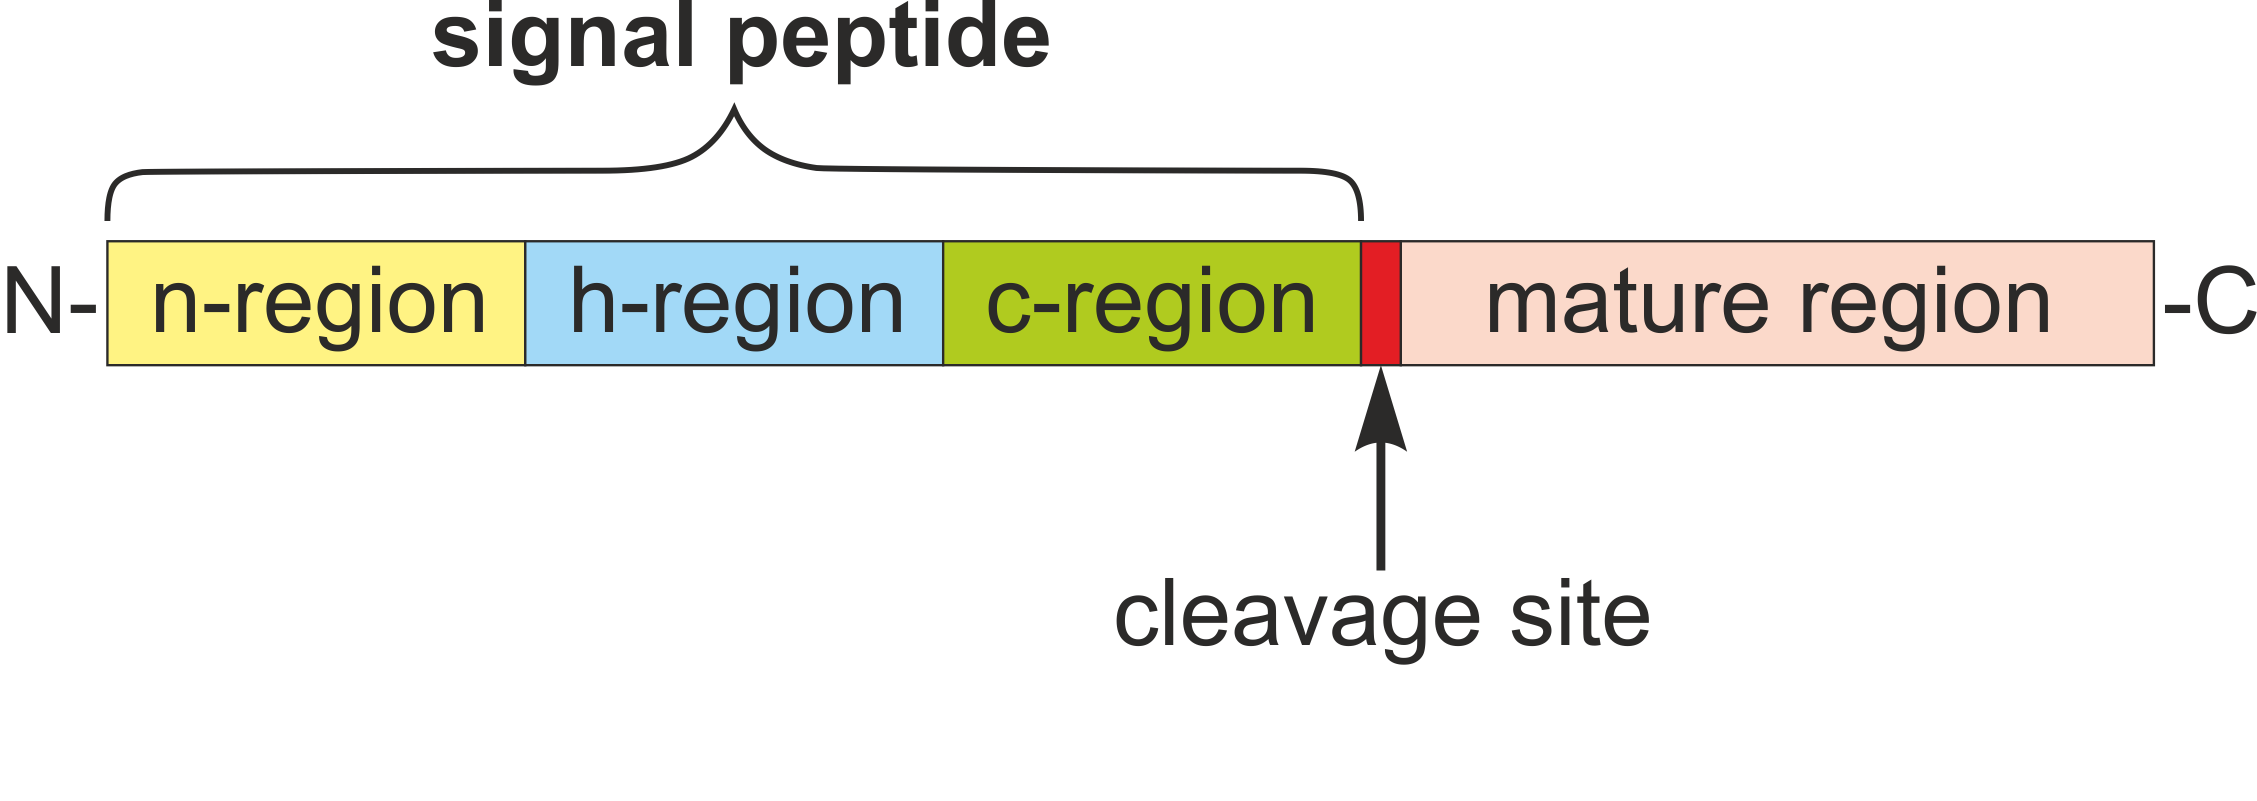
\includegraphics[width=0.5\textwidth]{SP.png}
\caption{The structure of signal peptide.}
\label{fig:sparch}
\end{figure}

\subsection*{Data selection}

Eukaryotic protein sequences and their annotations were properly prepared according to the literature of the subject and downloaded from UniProt database release 2015\_06. The positive set contained 2589 sequences with an experimentally confirmed signal peptide and its cleavage site. Sequences with more than one cleavage site were excluded from the final data set. The negative set comprised 152272 sequences without any signal peptide annotation. Protein sequences with ambiguous symbols: X, J, Z and B were removed from the final sets. Proteins with selenocysteine (U) were also excluded from data set, because there are no records of signal peptides containing this amino acid.

\subsection*{Clustering of amino acids}

Amino acids were clustered using several criteria relevant for the architecture of signal peptide: hydrophobicity, frequency in alpha-helices, polarity and size. High values of hydrophobicity are required in the h-region, the core of signal peptides. Alpha-helix, the secondary structure of this region, is probably induced by the positively charged n-region. Polarity as well as size are important especially in the cleavage site~\citep{1994palzkillselection}.

\begin{table}[ht]
\centering
\begin{tabular}{ll}
  \toprule
Criterion name & Property name \\ 
  \midrule
Size & Size \\ 
   \rowcolor[gray]{0.85}Size & Molecular weight \\ 
  Size & Residue volume \\ 
   \rowcolor[gray]{0.85}Size & Bulkiness \\ 
  Hydrophobicity & Normalized hydrophobicity scales for alpha-proteins \\ 
   \rowcolor[gray]{0.85}Hydrophobicity & Consensus normalized hydrophobicity scale \\ 
  Hydrophobicity & Hydropathy index \\ 
   \rowcolor[gray]{0.85}Hydrophobicity & Surrounding hydrophobicity in alpha-helix \\ 
  Polarity & Polarity \\ 
   \rowcolor[gray]{0.85}Polarity & Mean polarity \\ 
  Frequency in alpha-helices & Signal sequence helical potential \\ 
   \rowcolor[gray]{0.85}Frequency in alpha-helices & Normalized frequency of N-terminal helix \\ 
  Frequency in alpha-helices & Relative frequency in alpha-helix \\ 
   \bottomrule
\end{tabular}
\caption{Properties used in clusterization.} 
\label{tab:aaprop}
\end{table}

We selected 13 properties from AAIndex database (aaindexcitation) (see Table~\ref{tab:aaprop}), each attributed to a single criterion. Considering all combinations of single properties for every criterion, we created 96 possible clusterings of amino acids using Euclidean distance and Ward's method. 

To compare encodings we performed a 5-fold cross-validation training a new instance of signalHsmm on every encoding. We created balanced data sets by subsampling a number of proteins without a signal peptide equal to the number of proteins with signal peptide. The cross-validation was repeated XXX times, to ensure that every negative protein was tested at least once with XXX probability.

\subsection*{Hidden semi-Markov model}

Tu troche matematyki o ukrytych modelach Markova.


\section*{Results}

You may want to separate results, discussion and conclusion, according to your needs.

Please submit the final pdf file via EasyChair to the GCB'15 program committee by June 30, 2015. 

\section*{Discussion}

\section*{Acknowledgments}
Thank you for your support!


\bibliography{lokalizom}

\end{document}
